\documentclass[fleqn,10pt]{./class/wlscirep}
\title{Analizing resource allocation for a distributed monitoring application}

\author[1,2,3,*]{Bogdan-Constantin Irimie}

\affil[1]{Institute e-Austria Timisoara, Romania}
\affil[2]{Department of Computer Science, West University of Timisoara, Romania}
\affil[3]{Department of Computing, Imperial College London, United Kingdon}
\affil[*]{bogdan.irimie90@e-uvt.ro}

\keywords{Resource allocation, performance monitoring}

\begin{abstract}
In a cloud environment monitoring applications should be able to scale in order to satisfy the monitoring requirements offering good quality of service and efficient resource utilization. In order for this scaling to be possible, monitoring applications should be built from the ground up with this goal in mind and mechanism for auto scaling should be implemented in order to provide a fast adaptation time. This report describes the work that has been done in order to enhance a monitoring system with automatic resource allocation capabilities. The work describes possible architectures with their advantages and drawbacks and implementations with their technical challenges.
\end{abstract}
\begin{document}

\flushbottom
\maketitle
\thispagestyle{empty}

\section*{Introduction}

Monitoring plays an important role in todays offerings of computing computing because it enables cloud providers and consumers to check if the quality of service they have agreed upon is satisfied, additionally monitoring can be used to verify that a certain level of security is enabled. 

Resources in the cloud can be provisioned and released with ease in a short period of time and monitoring systems should be able to scale just as fast in order to adapt to the new monitoring requirements. In order to adapt, the monitoring systems
should relay on a resource allocation mechanism that can take into account the architectures of the monitoring systems and provide strategies for resource allocation. The architecture of the monitoring systems is very important because it dictates the means of obtaining scalability, some systems having architectures that allow scaling with ease by providing decoupled systems where each component can be scaled independently,while other systems are build on a monolithic architecture making scaling more challenging and in some cases even impossible.

In this report we will focus on a monitoring system that implements a pipe and filter architecture allowing independent scaling of all components, and thus providing fault tolerance and parallel execution of jobs. 

\section{Analyzing the system and it's architecture}

The architecture presented Fig. \ref{fig:systemArchitecture} of the system is an extension of [cite paper from SYNASC]. The system is composed of 7 components: FrontEnd, Scanner, Converter, Presenter, Remediator, a document database and a message queue. The first five components send messages using the queue and are completely decoupled from one another, from each component perspective the system is only compose of itself and one or more message queues. This decoupling provides grate opportunity for replication and scalability.

\section{The problem}
Although the system is very flexible and allows replication of components, it does not contain any component that is able to evaluate it's state and make decisions regarding allocation and release of resources consequently scaling must be done manually. Manual scaling the system can become a complex problem because each component has different resource requirements and even the same component can use more or less of a resource, depending on the job that it must execute. Monitoring the system manually and scaling it quickly become unmanageable and an automated way to do the scaling is desirable. 

In order to scale the system automatically, key performance metrics must be gathered and analyzed. 

\section{Gathering performance metrics}
Some of the basic performance parameters that can be gathered for a component are CPU, memory and network usage. Knowing the resource utilization of one component allows us to take decisions regarding deployment of that component. For example we can have 2 component, one with high CPU usage and one with high network usage, it would be wise to combine replicas of those components on the same VM or to allocate the ones that require high CPU usage to VM's with powerful CPU. By having this insight on component resource utilization we are able to take those decisions and to use the resources that we have in an efficient way. But resource utilization for components can vary with time, so a static scheme is not very useful, because it becomes outdated in a short period of time. Conterminous monitoring the components and taking actions on fresh performance metrics is crucial in guaranteeing optimal allocation strategies.

\subsection{Monitoring CPU}
 


\begin{figure}[ht]
\centering
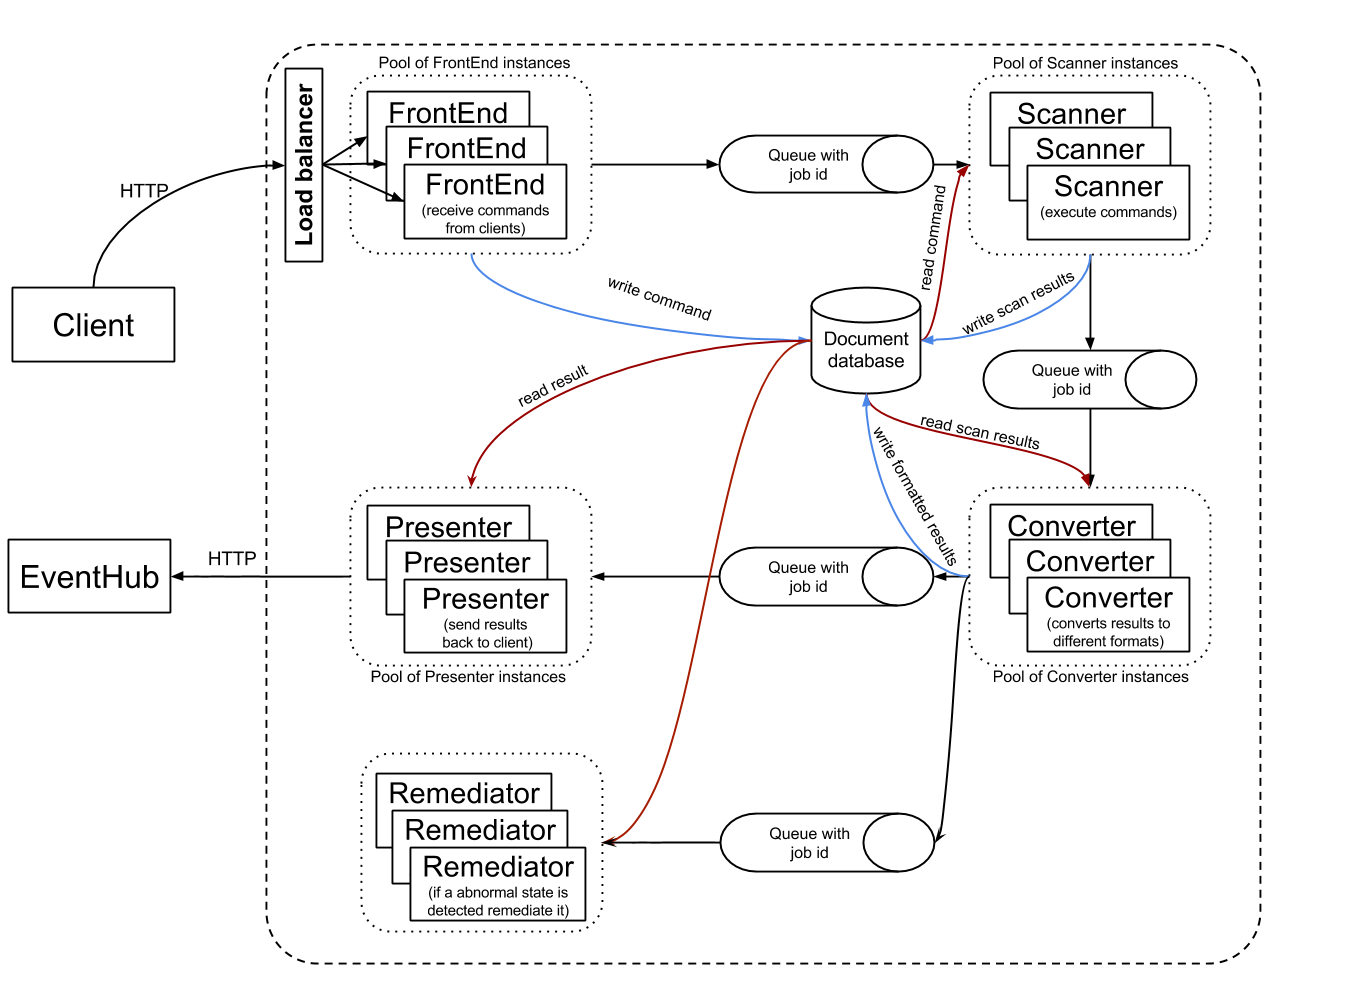
\includegraphics[width=\linewidth]{./img/MonitoringSystemArchitecture Remediation.png}
\caption{Distributed monitoring system architecture}
\label{fig:systemArchitecture}
\end{figure}



\bibliography{./bib/sample}

\section*{Acknowledgements}


\end{document}
